\chapter{Referencial Teórico}
\label{Referencial_Teorico}

\section{Arqueologia}%
A arqueologia é a ciência que estuda as culturas humanas através da recuperação, análise e interpretação dos vestígios materiais deixados por essas sociedades ao longo do tempo. Esses vestígios podem incluir artefatos, edificações, utensílios, entre outros elementos materiais que fornecem informações valiosas sobre os modos de vida, as práticas sociais e as organizações econômicas e políticas dos povos antigos. Conforme destaca \cite{funari2024arqueologia}, a arqueologia é essencial para a compreensão da história da humanidade, pois complementa e enriquece os dados obtidos por outras disciplinas, como a história e a antropologia, permitindo uma visão mais abrangente e detalhada das sociedades passadas. Assim, ao explorar os vestígios materiais, os arqueólogos contribuem significativamente para a reconstrução e preservação da memória coletiva, além de promover a valorização do patrimônio cultural.
Ao falar de arqueologia podemos nos deparar com várias formas de expressão, como por exemplo, a arte rupestre.
\subsection{Arte Rupestre}
%Falar sobre a definição(que é mais geral), falar sobre a toca da onça. sobre pictoglifos(que são as pinturas).



O termo “rupestre” tem origem no latim "rupestris”, derivado de “rupes”, que significa "rocha" ou “penhasco”. Assim, define-se como "Arte Rupestre” toda expressão gráfica, seja gravura ou pintura, que utiliza como suporte uma superfície rochosa, independentemente de suas características e dimensões \cite[p. 7]{pedroignacioschmitz_1984_arte}. As paredes de abrigos, grutas, penhascos e até mesmo rochas isoladas se transformam em telas para essas manifestações ancestrais.
Existem dois principais tipos de arte rupestre:
\begin{itemize}
\item \textbf{Pintura Rupestre (Pictografia):} Criação de imagens utilizando pigmentos minerais, vegetais ou animais, aplicados diretamente na superfície rochosa.
\item \textbf{Gravura Rupestre (Petróglifo):} Produção de desenhos através do desgaste da superfície rochosa, utilizando ferramentas líticas, como pedras pontiagudas.
\end{itemize}
A arte rupestre, presente em diversas partes do mundo, representa uma das formas mais antigas de expressão humana, oferecendo informações valiosas sobre as culturas que as produziram (MARQUES, 2016).

\subsection {Sítio Arqueológico Lapa da Pedra}\label{sec:sitio lapa da pedra}
O Sítio Arqueológico Lapa da Pedra, mostrado na Figura \ref{fig:Entrada da Gruta IV,Toca da Onça}, é conhecido popularmente como Toca da Onça fica localizado em uma fazenda de propriedade privada a nordeste de Formosa, chamada fazenda Pedra. Na Figura \ref{fig:mapa} pode-se observar o mapa e o caminho percorrido. Em 1984, Pedro Ignácio Schmitz e Altair Sales Barbosa realizaram pesquisas que culminaram na identificação e catalogação de 29 pequenas grutas na região de Formosa, Goiás. Essas grutas abrigavam pinturas rupestres e serviram como moradia para os primeiros habitantes do cerrado (BARBOSA et al., 1984, 1993). 
Dentre as 29 grutas, a Gruta catalogada por Schmitz como IV–GO-EC-002 (04), se destaca pela maior concentração de pictoglifos e, portanto, foi o foco da virtualização neste trabalho. Localizada a cerca de 12 km da cidade de Formosa, a Gruta 04 consiste em uma passagem de duzentos metros abaixo de uma enorme pedra calcária, situada na fazenda Pedra. Esse sítio, semelhante a outros em Goiás e no noroeste de Minas Gerais, apresenta uma grande diversidade de temas na arte rupestre, datando de aproximadamente 4.560 a.C. (SCHMITZ, 1990).


\begin{figure}[H]
    \centering
    \includegraphics[height=11cm, keepaspectratio]{img/Entrada Gruta IV Toca da Onça.jpeg}
    \caption{Entrada da Gruta IV, Toca da Onça. \\
        \textbf{Fonte:} Elaborado pelo autor, 2024.}
    \label{fig:Entrada da Gruta IV,Toca da Onça}
\end{figure}

\begin{figure}[H]
    \centering
    \includegraphics[height=8cm, keepaspectratio]{img/Visitas tecnicas/mapa.png}
    \caption{ Diagrama em cima da captura de tela do Google Earth \\ na localização das grutas da Lapa da Pedra. Captura de tela realizada em junho de 2024 \\
        \textbf{Fonte:} Elaborado pelo autor, 2024.}
    \label{fig:mapa}
\end{figure}


\subsection{Ameaças à Preservação da Arte Rupestre: Deteriorização e Ação Antrópica}\label{sec:amecas a preservação}
A arte rupestre, como patrimônio cultural de valor inestimável, enfrenta diversos desafios para sua preservação. A ação do tempo e as condições climáticas, como a umidade, a luz, o calor e o vento, contribuem para a deterioração natural das pinturas e superfícies rochosas.
Na Toca da Onça,  não bate sol dentro da gruta, contribuindo para a preservação do estado dos desenhos. Contudo, ainda se observam fatores de deterioração natural: descamação da tinta, infiltrações, fissuras nas rochas.


Além da deterioração natural, a ação antrópica, que se configura como a interferência humana no ambiente, representa uma grave ameaça à preservação da arte rupestre. Vandalismo, turismo desordenado, contato direto com as pinturas, poluição e obras próximas aos sítios arqueológicos podem causar danos irreversíveis a este patrimônio.
Em relação à Toca da Onça, os seguintes exemplos de impactos causados pela ação antrópica foram notados: vandalismo, pichações, degradação causada pelo turismo desordenado, fotos com \textit{flash}. Como por exemplo o que pode ser observado na Figura \ref{fig:degradacao_toca_onca}.

\begin{figure}[H]
    \centering
    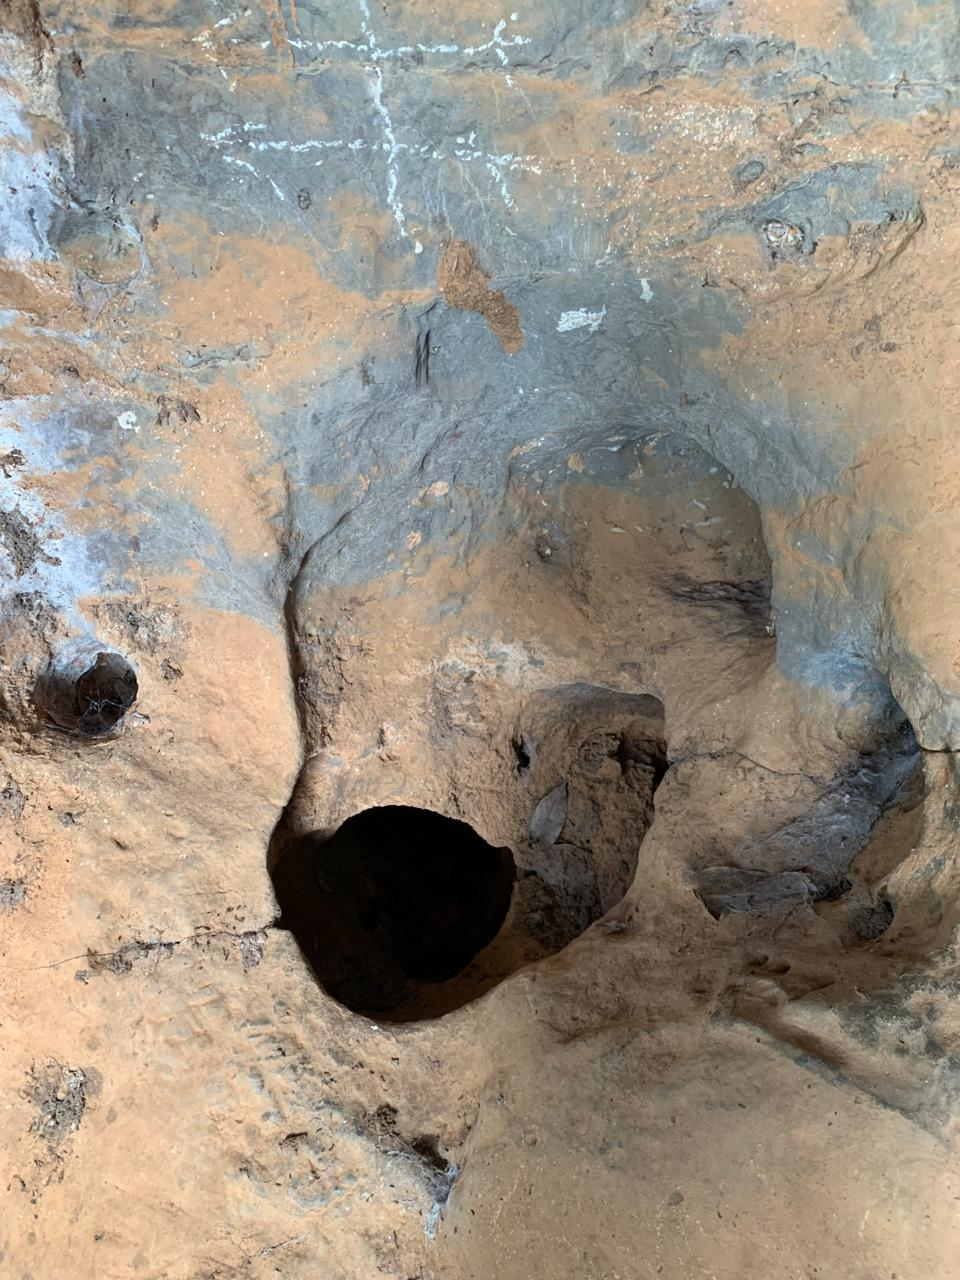
\includegraphics[height=11cm, keepaspectratio]{img/jogo da velha.jpeg}
    \caption{Depredação do Patrimônio na Toca da Onça. \\
        \textbf{Fonte:} Elaborado pelo autor, 2024.}
    \label{fig:degradacao_toca_onca}
\end{figure}


\section{Patrimônio Virtual (Virtual Heritage)}
\subsection{Conceitos e Importância}
Discutir o conceito de patrimônio virtual e seu impacto na arqueologia.

Diante dos desafios para a preservação da arte rupestre, a virtualização 3D surge como uma ferramenta poderosa para documentar, estudar e divulgar este importante patrimônio cultural, minimizando os impactos causasdos da visitação aos sítios arqueológicos.

\subsection{Aplicações em Arqueologia}
Dar exemplos de como o patrimônio virtual tem sido usado para preservar sítios históricos.




\section{Fotogrametria e Modelagem 3D}\label{sec:fotogrametria e modelagem 3D}
Para construção de um Patrimônio Virtual com qualidade é preciso construir modelos 3D fidedignos a realidade e para isso existe uma técnica muito utilizada chamada fotogrametria.
A fotogrametria, deriva das raízes gregas “photós” (luz), “gramma” (desenhado ou escrito) e “metria” (medição). Logo, fotogrametria etimologicamente significa “medições gráficas por meio da luz" (Paredes, 1987). A American Society for Photogrammetry and Remote Sensing (ASPRS), em seu livro The Manual of Photogrammetry (2003), define fotogrametria como “a arte, ciência e tecnologia de obter informações confiáveis sobre objetos físicos e o ambiente por meio de processos de registro, medição e interpretação de imagens fotográficas e padrões de energia radiante eletromagnética (EM) e outros fenômenos.”
Historicamente, a fotogrametria  teve seu desenvolvimento intrinsecamente ligado à evolução da fotografia, da óptica e da geometria, culminando em uma ferramenta crucial para diversos campos do conhecimento. No Brasil, sua história acompanha de perto a evolução global, com momentos de pioneirismo e adaptação às demandas nacionais (Silva, 2015).

Quanto a sua evolução, a fotogrametria passou por quatro fases principais: a Fotogrametria de Tábua Plana (1850–1900), iniciada por A. Laussedat com o uso de fotografias terrestres para mapeamento (Silva e Borges, 2023); a Fotogrametria Analógica (1900–1950), que incorporou a estereoscopia e fotografias aéreas para fins topográficos; a Fotogrametria Analítica (1950-1990), que otimizou os processos com a introdução de computadores e automatização; e a Fotogrametria Digital (1990-atualmente), caracterizada por processos automáticos realizados em computadores, além da popularização de câmeras digitais de alta qualidade que simplificam o processo (Borges e Silva, 2023).

A criação de um modelo 3D com fotogrametria digital, como descrito por Linhares e Groetelaars (2021), envolve um processo que se inicia com o planejamento do levantamento, definindo os objetivos, escolhendo o equipamento adequado e planejando a tomada fotográfica. A etapa seguinte, como apresentado por Groetelaars (2004), é a aquisição de dados no campo, que consiste na captura de fotografias e na medição das coordenadas dos pontos de controle no espaço real, utilizando métodos topográficos ou 3D Laser Scanning. Após a aquisição, o processamento dos dados é realizado por softwares específicos, que orientam as imagens interna e externamente com base nos pontos de controle, gerando uma nuvem de pontos densa. A partir dessa nuvem, o software cria uma malha triangular irregular (TIN), que representa a forma do objeto e pode ser texturizada com as imagens originais. A etapa final envolve o pós-processamento para remover ruídos, \textit{outliers} e falhas, otimizar a malha e aplicar texturas, resultando em um modelo 3D fotorrealístico.
A fotogrametria automatizada, comumente empregada na geração de modelos 3D de sítios arqueológicos, envolve um processo que se inicia com a captura de imagens de alta qualidade, utilizando câmeras terrestres ou aéreas com sobreposição e georreferenciamento por meio de pontos de controle (GCPs) (McGlone, 2004). O software realiza o alinhamento das imagens, corrigindo distorções geométricas e determinando a posição e orientação de cada fotografia no espaço. Através da correlação de imagens, o software identifica pontos correspondentes e calcula as coordenadas 3D de cada ponto, gerando uma nuvem densa de pontos 3D (Heipke, 2001). A partir da nuvem de pontos, o software gera modelos 3D, atribui texturas e corrige distorções geométricas, produzindo modelos 3D precisos e realistas do sítio arqueológico (Gruen, 2008). A geração de modelos 3D permite a documentação detalhada do sítio, a análise tridimensional da estrutura e a criação de representações visuais para estudos e divulgação científica.


%\subsection{Engine}
\subsection{Unreal Engine}No contexto do desenvolvimento de jogos e aplicações interativas, a \textit{engine} desempenha um papel fundamental como a espinha dorsal tecnológica. Uma \textit{engine} de jogo é um conjunto complexo de bibliotecas de software que fornece aos desenvolvedores um arcabouço completo para criar e alimentar experiências interativas em tempo real. Essas ferramentas abrangem desde a renderização gráfica e simulação de física até a inteligência artificial, interface do usuário e gerenciamento de áudio. Sem uma \textit{engine}, os desenvolvedores precisariam construir todas essas funcionalidades do zero, tornando o processo de desenvolvimento significativamente mais complexo e demorado. 

A \textit{Unreal Engine}, desenvolvida pela\textit{ Epic Games}, se destaca como uma \textit{engine} de jogos de última geração, amplamente utilizada na indústria de jogos e simulações, e reconhecida por sua capacidade de criar experiências visuais de alta qualidade e interativas.  A \textit{Unreal Engine} oferece um conjunto robusto de ferramentas para modelagem 3D, animação, física, renderização, iluminação, realidade virtual e muito mais. Sua arquitetura flexível e código-fonte aberto permitem que os desenvolvedores personalizem e estendam a \textit{engine} para atender às necessidades específicas de seus projetos, tornando-a uma escolha popular tanto para grandes estúdios quanto para desenvolvedores independentes.

No âmbito do Patrimônio Virtual, a \textit{Unreal Engine} se torna uma ferramenta poderosa para a criação de reconstruções digitais imersivas e interativas de sítios arqueológicos, monumentos e artefatos históricos. A \textit{engine} permite a modelagem 3D realista, a aplicação de texturas detalhadas e a simulação precisa de iluminação, proporcionando aos usuários uma experiência virtual imersiva e próxima da realidade. A capacidade de integrar elementos interativos, como navegação em primeira pessoa, animações e informações contextuais, enriquece ainda mais a experiência, tornando a \textit{Unreal Engine} uma escolha estratégica para projetos que buscam aproximar o público do patrimônio cultural.

\subsection{RealityCapture e Integração com Unreal Engine}
O \textbf{RealityCapture}, desenvolvido pela CapturingReality e adquirido pela Epic Games, é amplamente utilizado para a criação de modelos 3D altamente detalhados a partir de técnicas de fotogrametria. Uma das principais vantagens do RealityCapture é sua integração nativa com a Unreal Engine, também desenvolvida pela Epic Games. Essa compatibilidade facilita a exportação de modelos 3D para a Unreal Engine, onde podem ser utilizados na criação de ambientes virtuais realistas, como em jogos, simulações ou experiências de realidade virtual (VR) \citep{EpicGamesDocs}.

A integração entre o RealityCapture e a Unreal Engine é particularmente útil em projetos de patrimônio cultural, onde a reconstrução digital de sítios arqueológicos ou artefatos pode ser visualizada em ambientes virtuais interativos. Essa combinação permite a criação de experiências imersivas, como visitas virtuais a museus ou sítios históricos, com um alto nível de realismo e detalhamento \citep{ExemploArtigo}.
\subsection{Metahumans}

A representação humana em ambientes virtuais tem papel crucial na criação de experiências imersivas e relacionáveis. No contexto do Patrimônio Virtual, a presença de personagens virtuais humanoides pode auxiliar na comunicação de narrativas históricas, guiar usuários por sítios arqueológicos reconstruídos e demonstrar costumes e atividades do passado. Nesse sentido, a ferramenta \textit{MetaHuman Creator} (Figura \ref{fig:metahuman creator}), da Epic Games, surge como um recurso poderoso para a criação de avatares digitais de alta fidelidade.
O \textit{MetaHuman Creator} permite a geração e personalização de rostos e corpos humanos com alto nível de realismo, incluindo detalhes como textura de pele, cabelo, expressões faciais e diferentes tipos de corpo. A interface intuitiva e a ampla gama de opções de personalização permitem a criação de personagens únicos e específicos, evitando a aparência genérica frequentemente associada a avatares digitais. Esse recurso permite a criação detalhada de personagens realistas que podem ser integrados em simulações e experiências interativas, enriquecendo a representação do patrimônio cultural, tornando-a mais próxima e humanizada.

\begin{figure}[H]
    \centering
    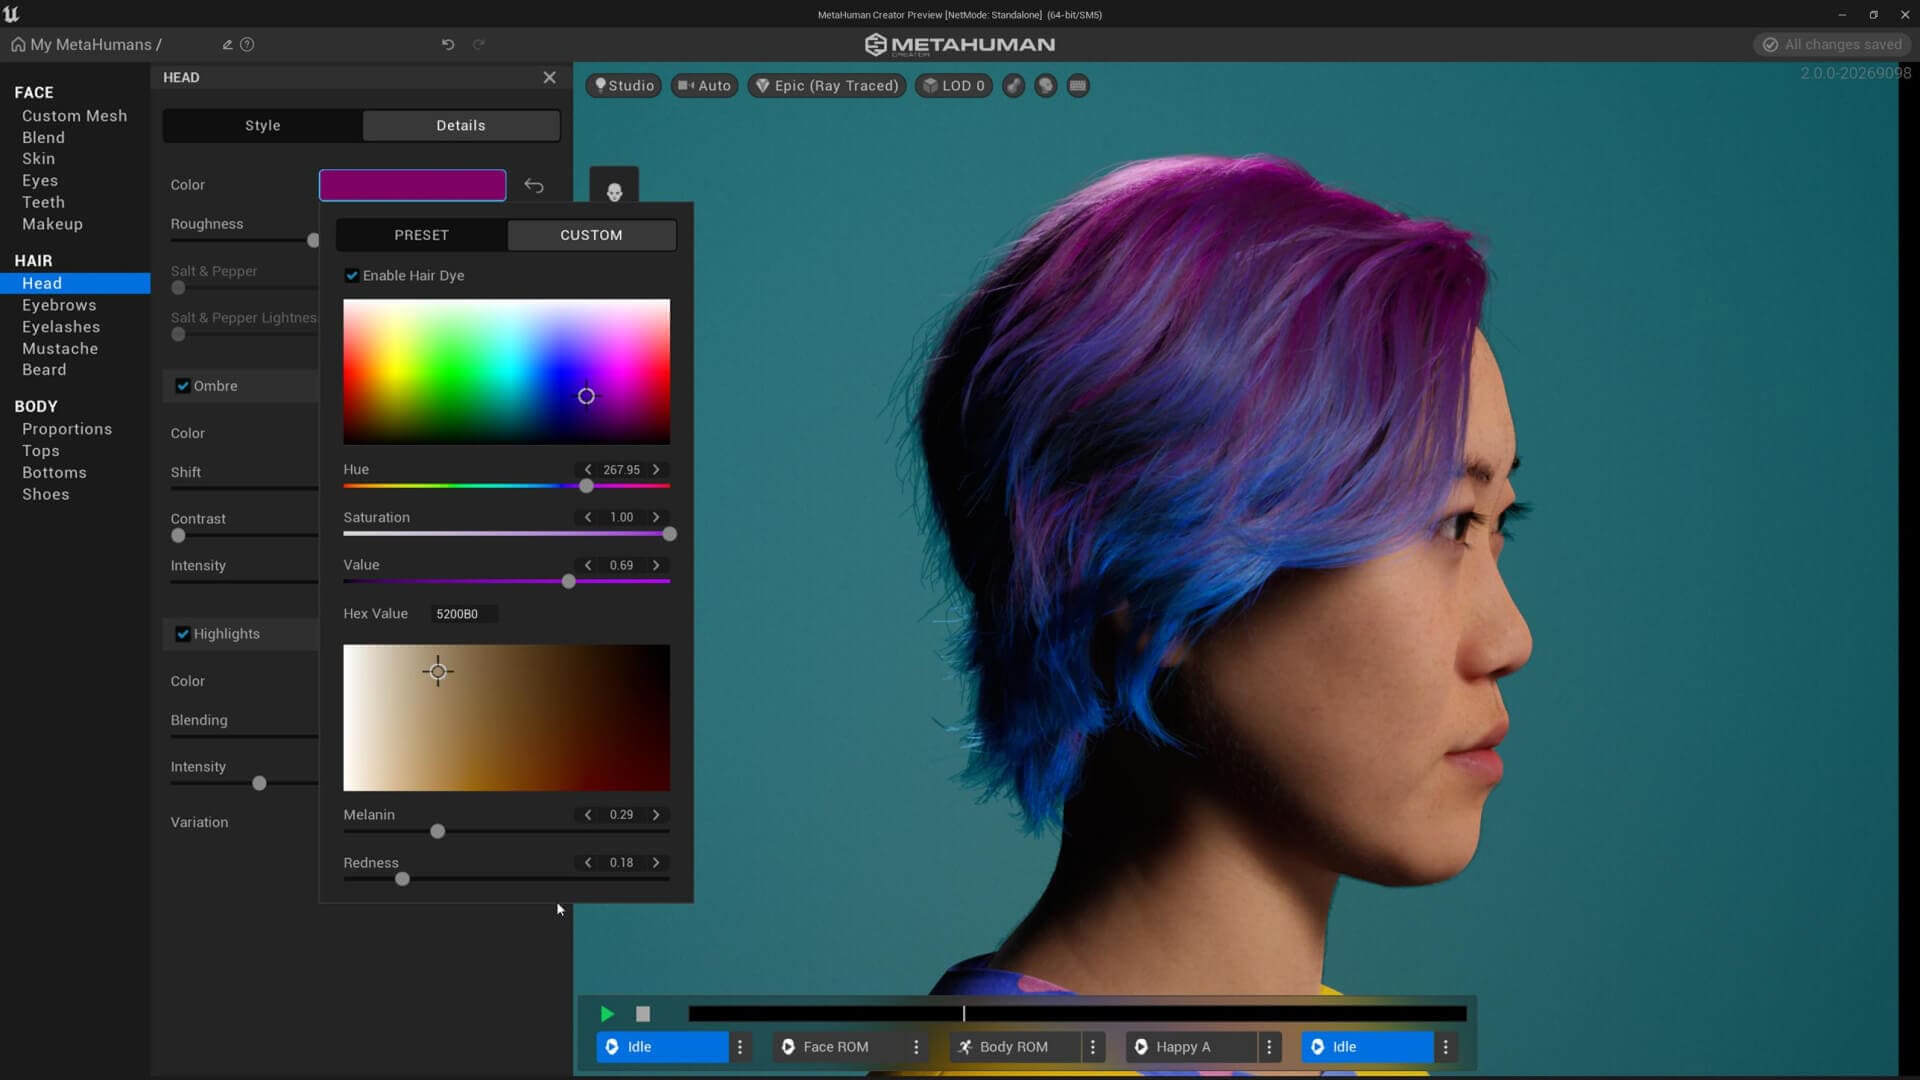
\includegraphics[height=8cm, keepaspectratio]{img/unreal/metahuman create.jpg}
    \caption{Editor da Plataforma MetaHuman \\
        \textbf{Fonte:} \href{https://cdn2.unrealengine.com/metahuman-overview-create-1920x1080-baa630fe8b02.jpg?resize=1&w=900}{Unreal Engine - MetaHumans},  \protect\citep{unrealenginemeta}}
    \label{fig:metahuman creator}
\end{figure}

Um aspecto fundamental para a integração convincente de Metahumans em ambientes virtuais é a animação. Cada \textit{MetaHuman} possui um "esqueleto digital" interno, uma estrutura articulada que permite a aplicação de movimentos, como mostrado na Figura \ref{fig:skeleton}. Através da importação de animações pré-definidas, que podem ser vistas na Figura \ref{fig:animacoes}, ou da criação de animações personalizadas utilizando softwares de animação 3D, é possível atribuir aos Metahumans ações como andar, correr, pular, gesticular e interagir com objetos no ambiente virtual. A fluidez e naturalidade dessas animações são essenciais para garantir a imersão do usuário e a credibilidade da representação.

\begin{figure}[H]
    \centering
    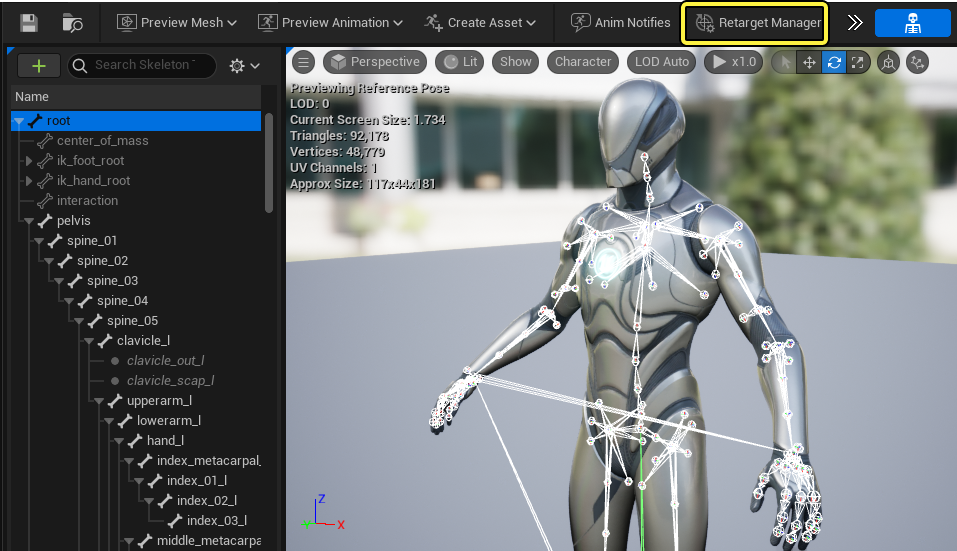
\includegraphics[height=8cm, keepaspectratio]{img/skeleton.png}
    \caption{Captura de tela do Esqueleto digital \\de um avatar na Unreal Engine.\\
        \textbf{Fonte:} Elaborado pelo autor, 2024.}
    \label{fig:skeleton}
\end{figure}

\begin{figure}[H]
    \centering
    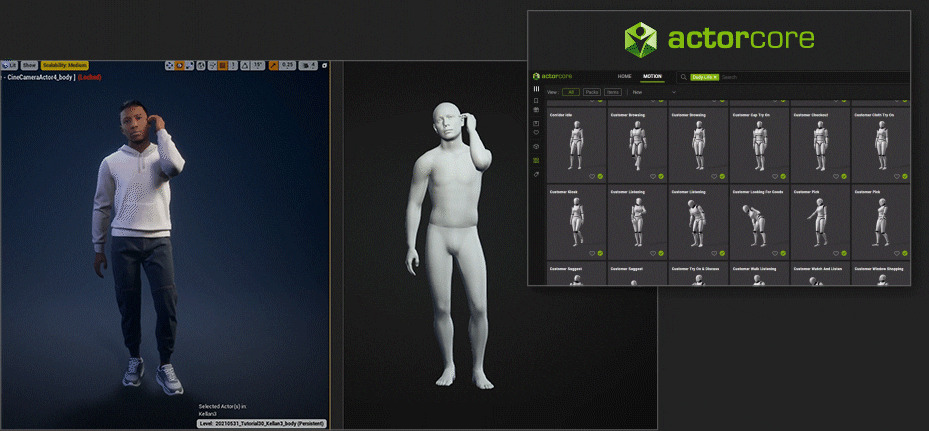
\includegraphics[height=8cm, keepaspectratio]{gif/animacoes/feature_body_motion-0000.jpg}
    \caption{ Captura de tela do pacote de animações Unreal.\\
        \textbf{Fonte:} Elaborado pelo autor, 2024.}
    \label{fig:animacoes}
\end{figure}


A Figura \ref{fig:metahumanEdson} ilustra a aplicação da tecnologia MetaHuman na representação do Professor Edson, profissional da área de artes e entusiasta da arqueologia. O modelo digital, criado a partir de fotografias como referência, captura suas características físicas com fidelidade, demonstrando o potencial da ferramenta na criação de representações personalizadas. A utilização de um MetaHuman com a aparência do Professor Edson em uma experiência de Patrimônio Virtual permite, por exemplo, que ele atue como um guia virtual, conduzindo os usuários por um sítio arqueológico reconstruído, fornecendo explicações e respondendo a perguntas, criando assim uma experiência mais interativa e humanizada.

\begin{figure}[H]
    \centering
    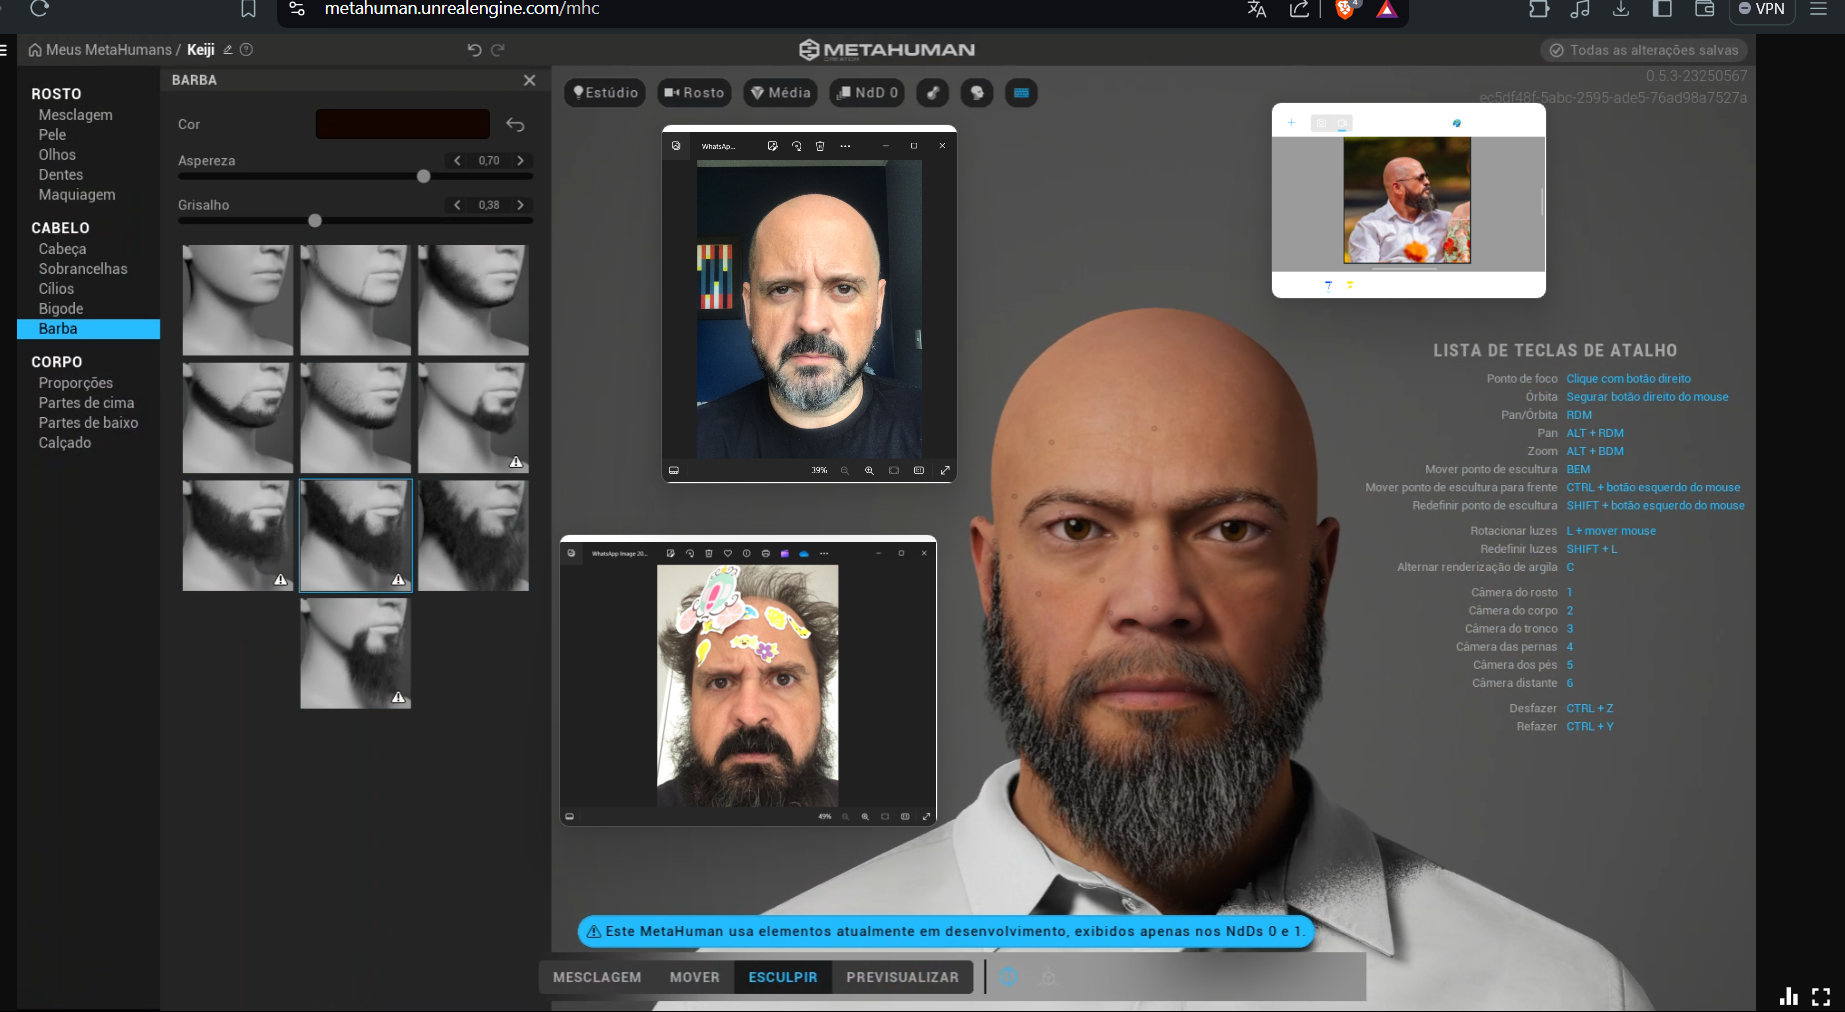
\includegraphics[height=8cm, keepaspectratio]{img/Metahuman.png}
    \caption{Criação do Avatar Digital do professor Edson Borges. \\
        \textbf{Fonte:} Elaborado pelo autor, 2024.}
    \label{fig:metahumanEdson}
\end{figure}



A capacidade de gerar personagens virtuais realistas e personalizáveis, combinada com a possibilidade de animá-los de forma natural e convincente, torna os Metahumans uma ferramenta poderosa para a criação de experiências imersivas e envolventes no campo do Patrimônio Virtual. A presença de personagens virtuais humanoides pode contribuir significativamente para a comunicação de narrativas históricas.

\section{Engenharia de Software}
% \subsection{Modelos de Processo}
% Discutir diferentes modelos de processo de desenvolvimento de software, como Cascata, Agile, etc.

\subsection{UML: Unified Modeling Language}
A Unified Modeling Language (UML) é uma linguagem de modelagem amplamente utilizada para visualizar, especificar, construir e documentar artefatos de sistemas de software \citep{Booch2005}. Criada por Grady Booch, James Rumbaugh e Ivar Jacobson, a UML oferece um conjunto de diagramas padronizados que auxiliam no entendimento e na comunicação entre equipes de desenvolvimento. Segundo \cite{Booch2005}, a UML é composta por diagramas estruturais (como Diagramas de Classe e de Objetos) e comportamentais (como Diagramas de Caso de Uso e de Sequência), que permitem representar diferentes perspectivas de um sistema.

A UML tem sido fundamental para a engenharia de software, especialmente no contexto de desenvolvimento orientado a objetos. Conforme destacado por \cite{Fowler2005}, a linguagem é flexível o suficiente para ser adaptada a diferentes metodologias de desenvolvimento, como o Rational Unified Process (RUP) e métodos ágeis. Além disso, a UML é mantida e atualizada pela Object Management Group (OMG), garantindo sua evolução contínua para atender às necessidades da indústria de software.

\subsection{Cenário de Caso de Uso}
Um cenário de caso de uso é uma descrição detalhada de uma sequência de interações entre um usuário (ou ator) e um sistema para alcançar um objetivo específico. Esses cenários são fundamentais na engenharia de software, pois ajudam a identificar e esclarecer os requisitos do sistema, garantindo que todas as possíveis interações sejam consideradas durante o processo de desenvolvimento \citep{pressman2021engenharia}.

\subsection{Requisitos Funcionais}
Requisitos funcionais especificam as funções que um sistema deve executar, descrevendo as entradas, comportamentos e saídas esperadas. Eles definem o que o sistema deve fazer para atender às necessidades dos usuários e são essenciais para orientar o desenvolvimento e a validação do software \citep{pressman2021engenharia}.

\subsection{Requisitos Não Funcionais}
Requisitos não funcionais referem-se às características de qualidade que o sistema deve possuir, como desempenho, segurança, usabilidade, confiabilidade e escalabilidade. Eles estabelecem restrições e critérios que influenciam a experiência do usuário e a eficácia do sistema, garantindo que o software atenda a padrões de qualidade além das funcionalidades básicas \citep{pressman2021engenharia}.

\section{Desenvolvimento Web}

O desenvolvimento web é uma área da tecnologia responsável pela criação, codificação e programação de sites, aplicativos e seus respectivos sistemas, envolvendo tanto aspectos visuais quanto funcionais \citep{queirosintrodução}. Este campo desempenha um papel essencial na democratização do acesso à informação e serviços digitais, permitindo que empresas, instituições e indivíduos alcancem públicos globais por meio da internet.

De acordo com QUEIRÓS E PORTELA (2018), o desenvolvimento web pode ser dividido em três áreas principais: \textit{front-end}, \textit{back-end} e \textit{full-stack development}. O \textit{front-end} refere-se à interface do usuário, ou seja, tudo o que o usuário visualiza e interage diretamente no navegador. Já o \textit{back-end} lida com a lógica do servidor, gerenciamento de dados e integração com bancos de dados. O \textit{full-stack development}, por sua vez, combina ambas as áreas, permitindo que um desenvolvedor trabalhe em todas as camadas de uma aplicação web.

No contexto deste projeto, optou-se por utilizar tecnologias modernas que refletem as tendências atuais do desenvolvimento web. Para o \textit{front-end}, foi adotado um \textit{framework} que facilita a criação de interfaces dinâmicas e responsivas, melhorando significativamente o desempenho e a otimização para mecanismos de busca (SEO). No \textit{back-end}, utilizou-se uma solução de gerenciamento de conteúdo (\textit{headless CMS}) que permite maior flexibilidade no design e na entrega de conteúdo, separando a camada de apresentação da camada de dados.

Os autores destacam que o desenvolvimento web moderno exige uma abordagem global, considerando tanto os aspectos técnicos quanto a experiência do usuário \citeP{queirosintrodução}. Essa perspectiva guiou as escolhas tecnológicas deste trabalho, priorizando desempenho, acessibilidade e facilidade de manutenção.

\section{Experiência do Usuário (UX)}
A Experiência do Usuário (UX) é um conceito fundamental no design de sistemas interativos, focando na satisfação e na eficiência do usuário ao interagir com um produto ou serviço. Segundo \cite{Norman}, UX abrange todos os aspectos da interação do usuário com uma interface, desde a usabilidade até a experiência emocional.

\subsection{Heurísticas de Nielsen}
As heurísticas de Nielsen, propostas por Jakob Nielsen em 1994, são um conjunto de princípios amplamente utilizados para avaliar a usabilidade de interfaces. Essas heurísticas servem como diretrizes para identificar problemas de usabilidade e melhorar a interação do usuário. A seguir, são apresentadas as 10 heurísticas de Nielsen:

\begin{enumerate}
    \item \textbf{Visibilidade do Status do Sistema}: O sistema deve sempre manter os usuários informados sobre o que está acontecendo, por meio de feedback adequado e em tempo razoável. Por exemplo, barras de progresso ou mensagens de carregamento são formas de fornecer feedback.

    \item \textbf{Correspondência entre o Sistema e o Mundo Real}: O sistema deve falar a linguagem do usuário, com palavras, frases e conceitos familiares, em vez de termos técnicos. As informações devem aparecer em uma ordem natural e lógica.

    \item \textbf{Controle e Liberdade para o Usuário}: Os usuários frequentemente realizam ações por engano e precisam de uma "saída de emergência" claramente marcada para sair do estado indesejado. Isso inclui funcionalidades como "Desfazer" e "Refazer".

    \item \textbf{Consistência e Padrões}: Os usuários não devem se perguntar se palavras, situações ou ações diferentes significam a mesma coisa. Siga as convenções da plataforma e mantenha a consistência em todo o sistema.

    \item \textbf{Prevenção de Erros}: Um bom design evita que problemas ocorram. Isso pode ser feito eliminando condições propícias a erros ou verificando se há erros antes que o usuário confirme uma ação.

    \item \textbf{Reconhecimento em vez de Memorização}: Minimize a carga de memória do usuário, tornando objetos, ações e opções visíveis. O usuário não deve precisar lembrar informações de uma parte do sistema para outra.

    \item \textbf{Flexibilidade e Eficiência de Uso}: Aceleradores (como atalhos de teclado) podem aumentar a eficiência para usuários experientes, sem prejudicar a experiência de usuários iniciantes.

    \item \textbf{Estética e Design Minimalista}: As interfaces não devem conter informações irrelevantes ou raramente necessárias. Cada unidade extra de informação compete com as unidades relevantes e diminui sua visibilidade relativa.

    \item \textbf{Ajudar os Usuários a Reconhecer, Diagnosticar e Recuperar-se de Erros}: As mensagens de erro devem ser expressas em linguagem simples, indicar precisamente o problema e sugerir uma solução de forma construtiva.

    \item \textbf{Ajuda e Documentação}: Embora seja melhor que o sistema possa ser usado sem documentação, pode ser necessário fornecer ajuda e documentação. Essas informações devem ser fáceis de encontrar, focadas na tarefa do usuário e listar etapas concretas a serem seguidas.
\end{enumerate}

Essas heurísticas são amplamente utilizadas em avaliações de usabilidade, como inspeções heurísticas, para identificar problemas em interfaces e propor melhorias \citep{Nielsen1994}.

\subsubsection{Análise Heurística}
A \textbf{Análise Heurística} é um método de avaliação de usabilidade que consiste na inspeção sistemática de uma interface com base em um conjunto de princípios ou heurísticas predefinidas. Esse método é amplamente utilizado para identificar problemas de usabilidade em sites, aplicativos e outros sistemas interativos, sem a necessidade de envolvimento direto dos usuários \citep{Nielsen1994}.
Os principais objetivos da análise heurística envolvem identificar problemas de usabilidade que possam prejudicar a experiência do usuário; avaliar a conformidade da interface com princípios de design reconhecidos, como as heurísticas de Nielsen; propor melhorias que aumentem a eficiência, a satisfação e a acessibilidade do sistema.

O processo de análise heurística geralmente é composto pelas etapas de:

\begin{enumerate}
    \item \textbf{Seleção das Heurísticas}: Escolha um conjunto de heurísticas adequado ao contexto da avaliação, como as heurísticas de Nielsen.
    
    \item \textbf{Inspeção da Interface}: Um ou mais avaliadores examinam a interface, aplicando as heurísticas selecionadas para identificar problemas de usabilidade.
    
    \item \textbf{Documentação dos Problemas}: Cada problema identificado é documentado, descrevendo sua natureza, a heurística violada e, se possível, sugerindo uma solução.
    
    \item \textbf{Priorização e Relatório}: Os problemas são priorizados com base em sua gravidade e impacto na experiência do usuário, e um relatório detalhado é gerado para orientar as melhorias.
\end{enumerate}

\subsection{Web Content Accessibility Guidelines (WCAG)}

Outra coisa relacionada com a experiência de usuário é a acessibilidade, e para metrificar isso exitem as \textbf{Web Content Accessibility Guidelines (WCAG)}, desenvolvidas pelo \textbf{W3C}, que são padrões globais para acessibilidade digital, garantindo que interfaces sejam acessíveis a todos, incluindo pessoas com deficiências \citep{wcag21}. Organizadas em quatro princípios (\textbf{POUR}), as WCAG abordam:

\begin{itemize}
    \item \textbf{Perceivable (Perceptível)}: Conteúdo deve ser apresentado de forma acessível (ex.: alternativas textuais para imagens).
    \item \textbf{Operable (Operável)}: Interfaces devem ser navegáveis por teclado e compatíveis com tecnologias assistivas.
    \item \textbf{Understandable (Compreensível)}: Conteúdo e operação devem ser claros e previsíveis.
    \item \textbf{Robust (Robusto)}: Conteúdo deve ser compatível com diversas tecnologias.
\end{itemize}

As WCAG possuem três níveis de conformidade: \textbf{A} (mínimo), \textbf{AA} (recomendado) e \textbf{AAA} (ótimo). Sua adoção promove inclusão digital, conformidade legal e melhoria da experiência do usuário \citep{wcag21}.

% \subsection{Melhores Práticas}
% Discutir a relevância da acessibilidade, otimização para SEO e práticas comuns de segurança em aplicações web.


\section{JAMstack e Desenvolvimento Web Moderno}
\label{sec:jamstack}
A JAMstack é uma arquitetura moderna para desenvolvimento web que se baseia em três pilares principais: \textbf{JavaScript}, \textbf{APIs} e \textbf{Markup} \citep{jamstackorg}, como exemplificado na Figura \ref{fig:jamStack sigla}\footnote{Disponível em \href{https://cloudbytes.dev/snippets/what-is-jamstack-and-why-should-you-be-using-it}{https://cloudbytes.dev/snippets/what-is-jamstack-and-why-should-you-be-using-it}}. Essa abordagem promove a criação de sites rápidos, seguros e escaláveis, separando o front-end do back-end e utilizando serviços de terceiros para funcionalidades dinâmicas \citep{netlifyjamstack}.

\begin{figure}[H]
    \centering
    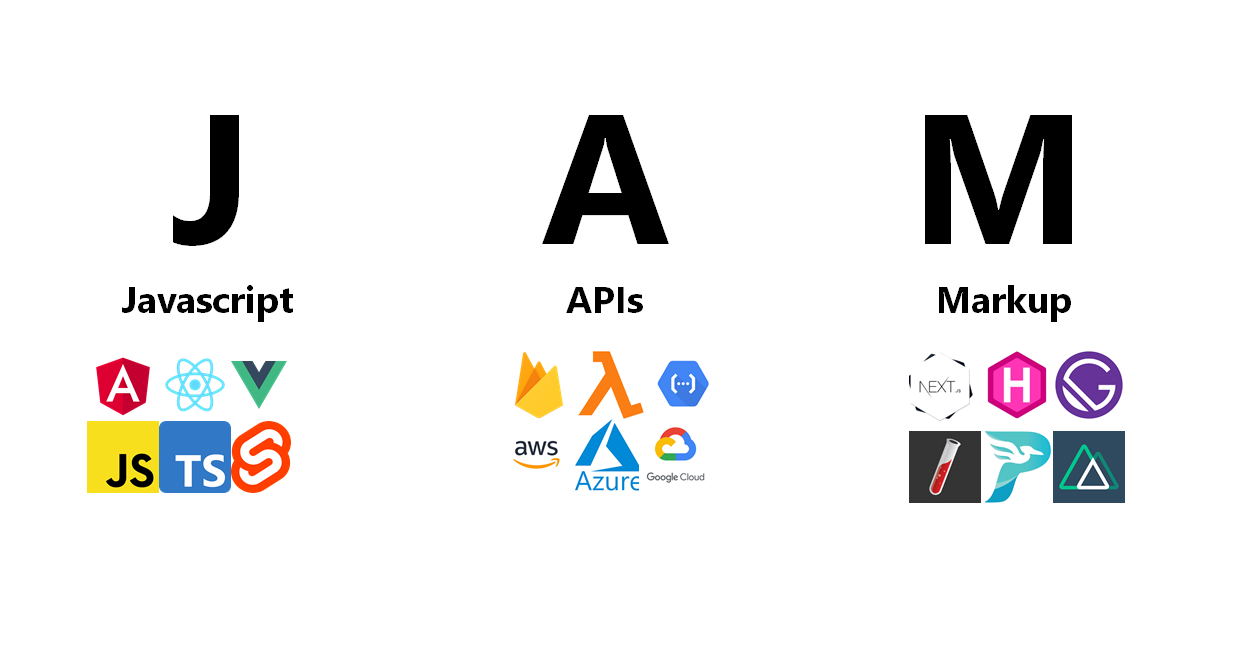
\includegraphics[height=8cm, keepaspectratio]{img/arquitetura/sigla JAM stack.png}
    \caption{ Significado da sigla JAM(Javascript, APIs e Markup)
 \\
        \textbf{Fonte:} Rehan Haider}
    \label{fig:jamStack sigla}
\end{figure}
De acordo com \cite{smashingmagazine}, a JAMstack tem ganhado popularidade devido à sua capacidade de simplificar o processo de desenvolvimento, permitindo que desenvolvedores se concentrem na experiência do usuário enquanto delegam tarefas complexas a APIs especializadas. Além disso, a pré-renderização de páginas estáticas contribui para uma melhor performance e segurança, reduzindo a superfície de ataque \citep{jamstackbook}.

A flexibilidade da JAMstack permite a integração com diversas ferramentas e serviços, como CMS headless, CDNs e ferramentas de automação, tornando-a uma escolha versátil para projetos de diferentes escalas \citep{netlifyjamstack}.

A arquitetura JAMstack (Figura \ref{fig:jamStack Arquitetura}) se destaca em relação a abordagens mais tradicionais, como o modelo de servidor monolítico e as arquiteturas baseadas em servidores dinâmicos. No modelo monolítico, todo o \textit{backend} e \textit{frontend} estão fortemente acoplados, exigindo que o servidor processe cada solicitação do usuário em tempo real. Isso pode gerar tempos de resposta mais lentos, especialmente em aplicações com alto tráfego, e torna mais difícil escalar ou implementar novas funcionalidades de maneira isolada.

\begin{figure}[H]
    \centering
    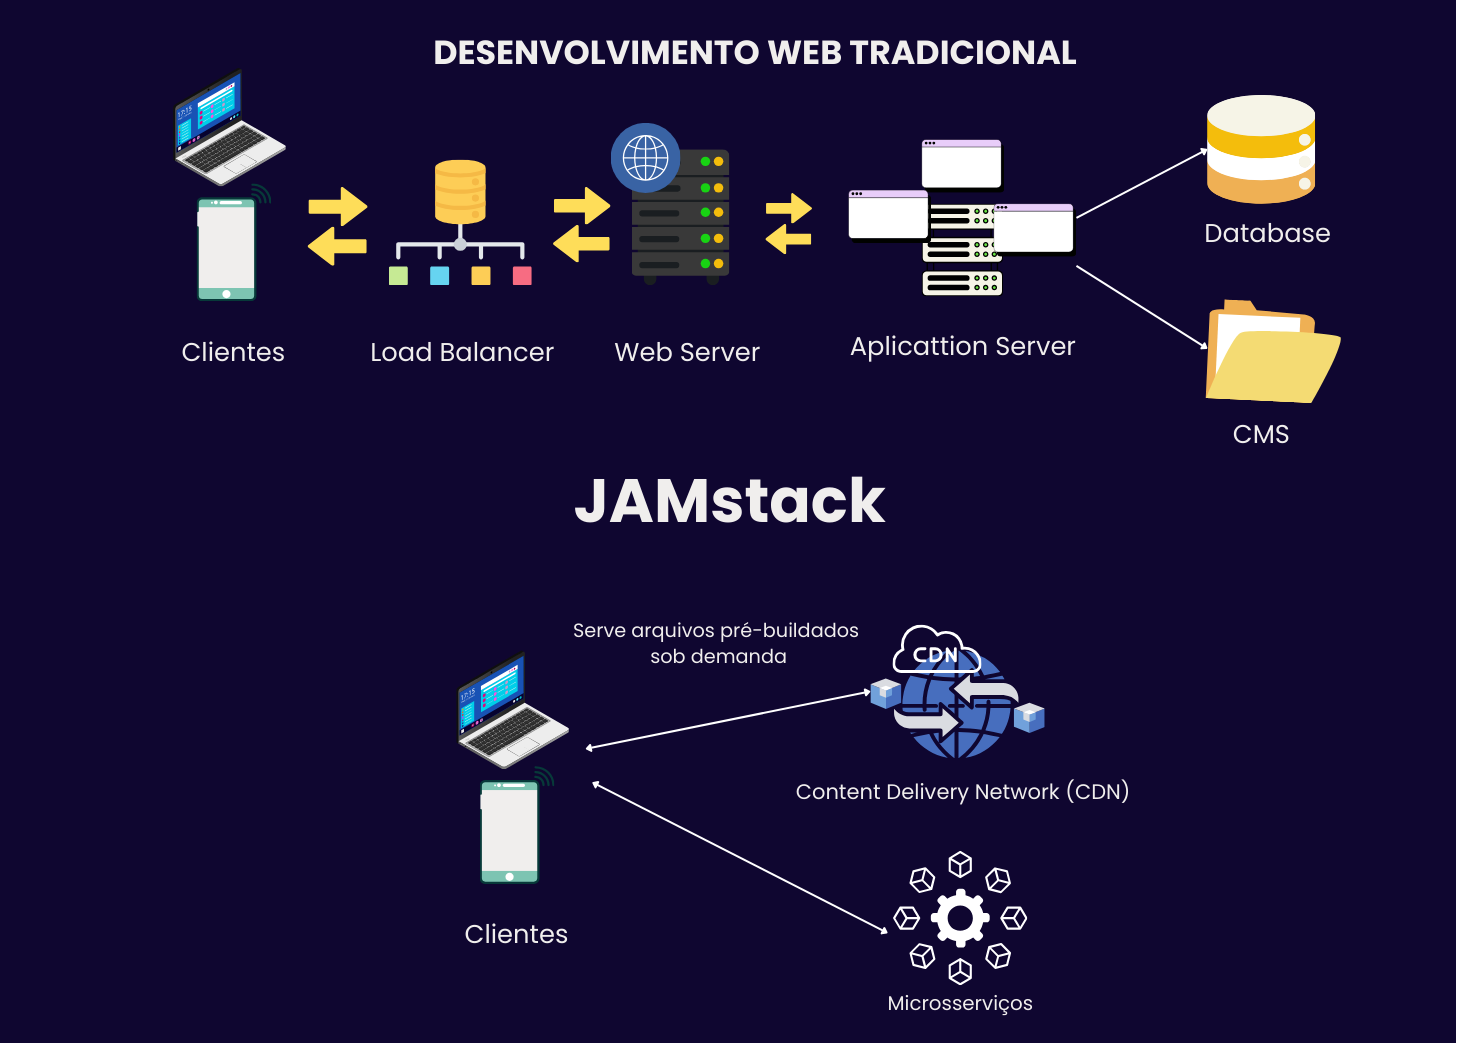
\includegraphics[height=8cm, keepaspectratio]{img/arquitetura/JAM STACK.png}
    \caption{ Comparação entre arquitetura tradicional e arquitetura JAMstack. \\
        \textbf{Fonte:} Elaborado pelo autor com base na documentação oficial do JAMstack, 2024.}
    \label{fig:jamStack Arquitetura}
\end{figure}

Já nas arquiteturas dinâmicas baseadas em servidores, como as utilizadas em sistemas gerenciadores de conteúdo tradicionais (ex.: WordPress), cada requisição ao site frequentemente aciona o servidor para buscar dados no banco e gerar a página no momento da requisição. Esse modelo pode causar problemas de performance e segurança, principalmente em picos de tráfego, além de depender de uma infraestrutura robusta para manter a operação.
Em contraste, a JAMstack evita a necessidade de renderização em tempo de execução, pré-gerando as páginas como arquivos estáticos no momento do build. Isso garante maior rapidez, segurança e escalabilidade, já que as páginas podem ser servidas diretamente por uma CDN sem passar por servidores intermediários. Além disso, ao desacoplar o \textit{frontend} do backend, a JAMstack permite maior flexibilidade, facilitando a integração com APIs e serviços especializados, como sistemas de pagamento ou autenticação.
Por outro lado, a JAMstack apresenta limitações quando comparada a arquiteturas como microserviços ou serverless, que também oferecem modularidade e flexibilidade. Embora APIs desempenhem um papel fundamental na JAMstack, aplicações com lógica de negócios altamente complexa podem exigir um \textit{backend} mais robusto, algo que arquiteturas serverless ou baseadas em microserviços conseguem oferecer de forma mais eficiente.

\section{Ferramentas Utilizadas}
Nesta seção, são apresentadas as principais ferramentas utilizadas no desenvolvimento deste trabalho, destacando suas funcionalidades e relevância para o projeto.

\subsection{Visual Studio Code}
O \gls{vs-code} é um editor de código-fonte desenvolvido pela Microsoft, amplamente utilizado por desenvolvedores devido à sua leveza, extensibilidade e suporte a diversas linguagens de programação. Ele oferece recursos como depuração integrada, realce de sintaxe, autocompletar inteligente e integração com ferramentas de controle de versão, como Git. Além disso, o VS Code possui um mercado de extensões que permite personalizar e expandir suas funcionalidades, tornando-o uma das ferramentas mais populares para desenvolvimento de software \citep{vscode}.

\subsection{Git e GitHub}
O Git é um sistema de controle de versão distribuído amplamente utilizado para rastrear alterações no código-fonte durante o desenvolvimento de software. Ele permite que desenvolvedores trabalhem em branches separados, facilitando a colaboração e a integração de mudanças. Já o GitHub é uma plataforma baseada em nuvem que hospeda repositórios Git, oferecendo funcionalidades adicionais como pull requests, issues e integração contínua. Juntos, Git e GitHub formam uma combinação poderosa para gerenciamento de projetos e colaboração em equipe \cite{git,github}.

\subsection{Notion}
 Notion é uma ferramenta de produtividade e organização que combina funcionalidades de notas, banco de dados, listas de tarefas e planejamento em uma única plataforma. Ele foi amplamente utilizado neste trabalho para a criação de quadros Kanban \footnote{Kanban é uma ferramenta de gestão visual que utiliza cartões para controlar tarefas e fluxos de atividades, permitindo maior organização e eficiência nos processos. O termo "Kanban" significa "sinalização" ou "cartão" e propõe o uso de post-its para indicar e acompanhar o andamento das atividades \citep{aguiar2007compreendendo}} e calendários (Figura \ref{fig:kanban notion}), permitindo o gerenciamento visual de tarefas e o acompanhamento do progresso do projeto. Além disso, o Notion foi empregado para o planejamento de etapas, organização de documentação e colaboração em equipe, graças à sua flexibilidade e integração de diferentes tipos de conteúdo em uma única interface. Sua capacidade de personalização e facilidade de uso o tornam uma ferramenta essencial para gestão de projetos e organização pessoal \citep{notion}.
 O Kanban nesse trabalho não foi utilizado como metodologia e sim como ferramenta auxiliar.
 A Figura \ref{fig:notion inicial} mostra a página inicial usada para organização e planejamento do TCC no Notion.

\begin{figure}[H]
    \centering
    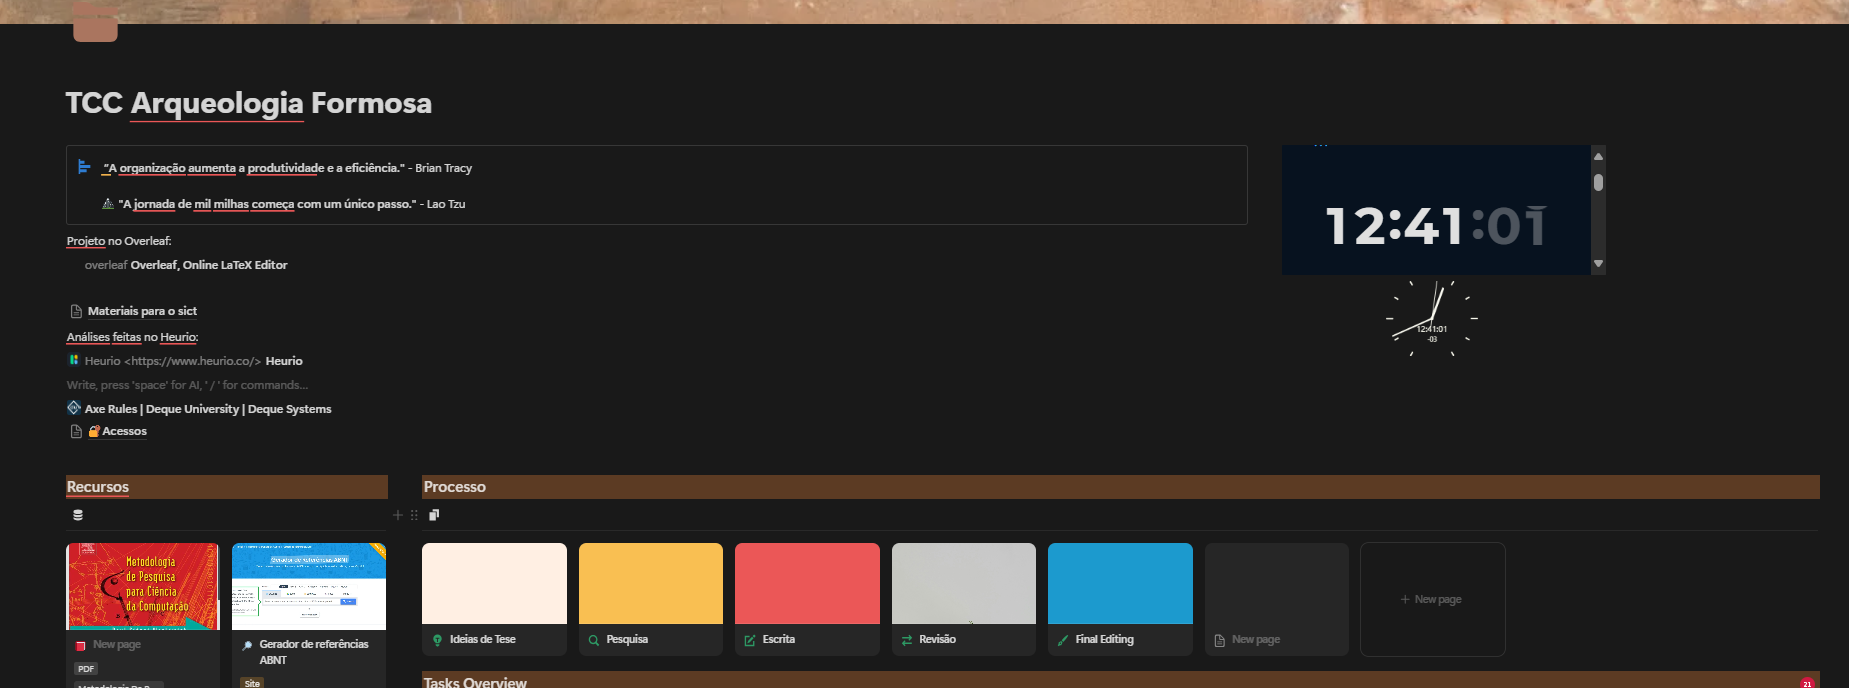
\includegraphics[height=6cm, keepaspectratio]{img/Notion/pagina inicial.png}
    \caption{ Página inicial do Notion para organização do TCC com etapas, \\ documentos úteis e ferramentas. \\
        \textbf{Fonte:} Elaborado pelo autor, 2024.}
    \label{fig:notion inicial}
\end{figure}

\begin{figure}[H]
    \centering
    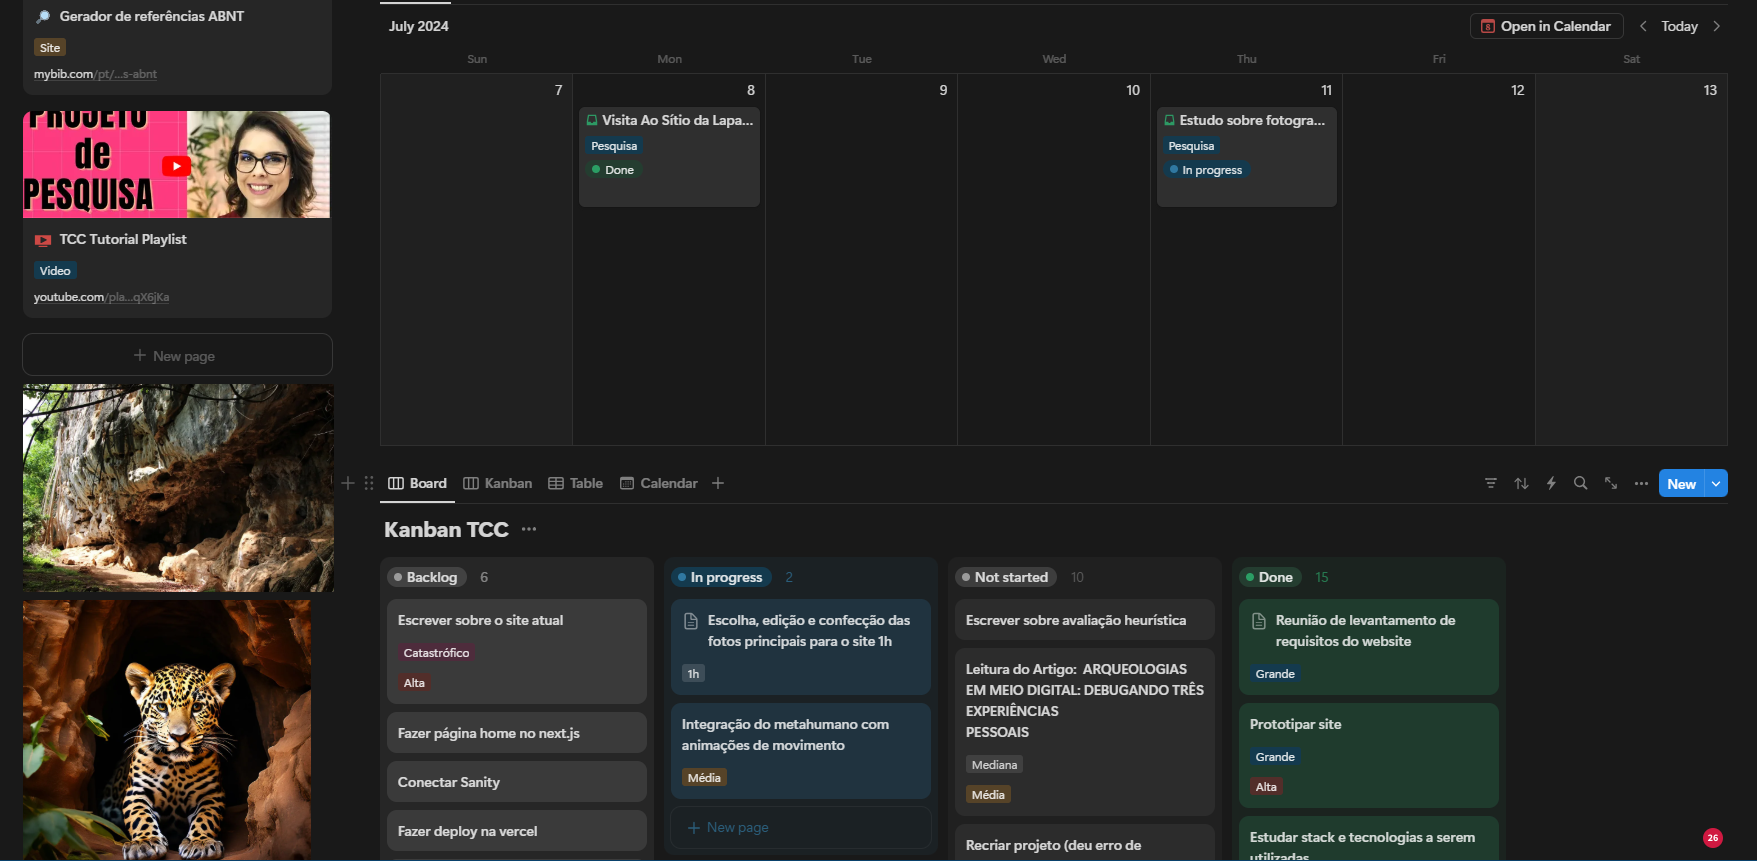
\includegraphics[height=8cm, keepaspectratio]{img/Notion/kanban.png}
    \caption{ Quadro Kanban e calendário para gerenciar atividades. \\
        \textbf{Fonte:} Elaborado pelo autor, 2024.}
    \label{fig:kanban notion}
\end{figure}


\subsection{Figma}
O Figma é uma ferramenta de design de interfaces baseada em nuvem, amplamente utilizada para criação de protótipos, designs colaborativos e sistemas de design. Ele se destaca por permitir que múltiplos usuários trabalhem simultaneamente em um mesmo projeto, facilitando a colaboração em tempo real. Além disso, o Figma oferece recursos como componentes reutilizáveis, autolayout e integração com outras ferramentas de desenvolvimento, tornando-o uma escolha popular entre designers e equipes de produto \citep{figma}.

% \subsection{Reality Capture}
% O \textbf{Reality Capture} é uma tecnologia de digitalização 3D que permite criar modelos tridimensionais altamente detalhados a partir de fotografias ou varreduras a laser. Essa ferramenta é amplamente utilizada em áreas como arquitetura, patrimônio cultural, produção cinematográfica e desenvolvimento de jogos, devido à sua capacidade de capturar objetos e ambientes reais com precisão e eficiência \citep{RealityCapture2023}.

% Uma das principais vantagens do Reality Capture é a sua precisão na reprodução de detalhes, o que o torna ideal para projetos que exigem fidelidade ao mundo real. Além disso, a tecnologia é eficiente, permitindo a digitalização de grandes estruturas ou objetos em um tempo relativamente curto. Os modelos gerados podem ser facilmente integrados a softwares de edição 3D e motores de jogos, como o Unreal Engine, o que amplia suas aplicações práticas \citep{RealityCapture2023}.

% No contexto de preservação do patrimônio cultural, o Reality Capture tem sido utilizado para digitalizar monumentos e sítios arqueológicos, garantindo que essas obras sejam preservadas digitalmente para futuras gerações. Na indústria de jogos e filmes, a ferramenta é empregada para criar assets 3D realistas, como personagens e cenários, que podem ser utilizados em produções de alta qualidade \citep{RealityCapture2023}.

% \subsection{Unreal Engine}
% A \textbf{Unreal Engine}, desenvolvida pela Epic Games, é um dos motores de jogo mais populares e versáteis do mercado. Conhecido por sua capacidade de renderizar gráficos de alta qualidade e suportar experiências interativas em tempo real, o Unreal Engine é amplamente utilizado não apenas no desenvolvimento de jogos, mas também em áreas como arquitetura, cinema e educação \citep{UnrealEngine2023}.

% Um dos recursos mais destacados do Unreal Engine é o sistema de \textit{Blueprints}, que permite a criação de lógica de jogo sem a necessidade de escrever código. Isso torna a ferramenta acessível para designers e artistas, que podem prototipar e desenvolver projetos de forma mais ágil. Além disso, o motor oferece suporte a tecnologias avançadas, como iluminação global e física realista, que contribuem para a criação de ambientes visualmente impressionantes \citep{UnrealEngine2023}.

% A integração do Unreal Engine com ferramentas como o Reality Capture é outro ponto forte. Modelos 3D gerados a partir de digitalizações do mundo real podem ser importados diretamente para o motor, onde podem ser manipulados e incorporados em projetos interativos. Essa combinação de tecnologias tem sido amplamente utilizada na criação de jogos realistas, simulações arquitetônicas e até mesmo em produções cinematográficas \citep{UnrealEngine2023}.

% Na área de educação, o Unreal Engine tem sido empregado para desenvolver simulações interativas e ambientes de aprendizagem imersivos. Sua flexibilidade e suporte a múltiplas plataformas, incluindo dispositivos móveis e realidade virtual, tornam-no uma escolha popular para projetos que exigem inovação e engajamento \citep{UnrealEngine2023}.

\subsection{Sanity}
O Sanity é um CMS (\textit{Content Management System}) headless\footnote{ Um Sistema de Gerenciamento de Conteúdo (CMS) é uma ferramenta ou plataforma que permite criar, gerenciar e organizar conteúdo digital, como textos, imagens e vídeos, sem a necessidade de conhecimento técnico avançado. Tradicionalmente, um CMS inclui tanto o \textit{backend} (onde o conteúdo é criado e armazenado) quanto o \textit{frontend} (onde o conteúdo é exibido). No caso de CMSs \textit{headless}, como o Sanity, o \textit{frontend} é desacoplado, permitindo maior flexibilidade na forma como o conteúdo é consumido e apresentado.} que se destaca por sua flexibilidade e arquitetura baseada em NoSQL, permitindo a criação de esquemas personalizados e facilitando a entrega de conteúdo em múltiplos canais digitais \citep{sanity_official}. Ele é frequentemente utilizado em conjunto com \textit{frameworks} modernos, como o Next.js, para criar soluções eficientes e escaláveis, onde o Sanity atua como \textit{backend} de conteúdo e o Next.js como \textit{frontend} responsivo e performático. Essa integração reflete uma abordagem contemporânea de desenvolvimento web, alinhada à ideia de sistemas modulares e desacoplados, conforme discutido por \cite{gamma2000padrões} que exploram a evolução das arquiteturas de software, além de funcionar muito bem com a arquitetura JAMstack. 


\subsection{Vercel}
A Vercel é uma plataforma de \gls{deploy} e hospedagem voltada para aplicações modernas, especialmente aquelas construídas com \glspl{framework} como Next.js, React e outros. Ela oferece integração contínua, escalabilidade automática e um desempenho otimizado para aplicações web estáticas e dinâmicas. Com foco na experiência do desenvolvedor, a Vercel simplifica o processo de publicação, permitindo que atualizações sejam feitas rapidamente através de integração com \gls{repositorio-git}. Sua infraestrutura global de \glsboth{cdn} garante baixa latência e alta disponibilidade para usuários finais \citep{vercel}.

\subsection{Heurio}
A extensão \textbf{Heurio} é uma ferramenta desenvolvida para auxiliar na realização de análises heurísticas de sites e interfaces digitais. Disponível como uma extensão para navegadores, o Heurio permite que profissionais de UX apliquem as heurísticas de usabilidade de forma prática e organizada, identificando problemas de usabilidade e propondo melhorias. \citep{Heurio}.

Dentre as funcionalidades do Heurio que facilitam a análise heurística estão:

\begin{itemize}
    \item \textbf{Lista de Heurísticas Integrada}: A extensão inclui uma lista de heurísticas de usabilidade, como as de Nielsen, que podem ser selecionadas e aplicadas diretamente durante a avaliação da interface.
    
    \item \textbf{Anotações e Comentários}: O Heurio permite que o avaliador faça anotações e comentários sobre problemas identificados, associando-os às heurísticas correspondentes. Isso facilita a documentação e a comunicação dos resultados.
    
    \item \textbf{Captura de Tela}: A ferramenta permite capturar telas da interface sendo avaliada, facilitando a visualização e a referência aos problemas encontrados.
    
    \item \textbf{Relatórios Automatizados}: Após a análise, o Heurio gera relatórios automatizados que organizam as anotações, capturas de tela e heurísticas aplicadas. Esses relatórios podem ser exportados e compartilhados com a equipe.
    
    \item \textbf{Colaboração em Equipe}: O Heurio suporta a colaboração entre múltiplos avaliadores, permitindo que equipes trabalhem juntas na mesma análise e compartilhem insights.
\end{itemize}

Essa ferramenta é particularmente útil em projetos de \textit{redesign} de sites, avaliação de protótipos e testes de usabilidade. Ela pode ser utilizada por equipes de \gls{ux}, designers e desenvolvedores para garantir que as interfaces atendam aos princípios de usabilidade e proporcionem uma experiência positiva ao usuário. Além disso, a ferramenta é flexível o suficiente para ser adaptada a diferentes contextos e metodologias de avaliação. \citep{Heurio}.

\subsection{Inno Setup}
O Inno Setup é um instalador gratuito para programas Windows, amplamente utilizado devido à sua facilidade de configuração e flexibilidade. Ele permite a criação de scripts de instalação personalizados, suportando recursos como criação de atalhos, registro de DLLs e desinstalação completa. Sua sintaxe é baseada em arquivos de texto no formato \texttt{.iss}, que são compilados para gerar executáveis de instalação. Por ser leve e de código aberto, o Inno Setup é uma escolha popular para desenvolvedores que buscam uma solução eficiente para distribuição de software \citep{innosetup}.